 \documentclass{article}
\usepackage{tikz}
\usetikzlibrary{positioning, automata}
\usepackage{fancyhdr}
\usepackage{extramarks}
\usepackage[plain]{algorithm}
\usepackage{algpseudocode}
\usepackage[utf8]{inputenc} 
\usepackage[T1]{fontenc}    
\usepackage{hyperref}       
\usepackage{url}        
\usepackage{booktabs}
\usepackage{pdfpages}
\usepackage{amsfonts}   
\usepackage{nicefrac}       
\usepackage{microtype}      
\usepackage{amsmath}
\usepackage{graphicx}
\usepackage{float}
\usepackage{caption}
\usepackage{ragged2e}
\usepackage{amssymb}
\usepackage{mathtools}
\usepackage{xcolor}
\usepackage[spanish]{babel} % ¡Solo una vez!
\usepackage{array}
\usepackage{multirow}
\usepackage{multicol}
\usepackage{manfnt}
\usepackage{layout}
\usepackage{manfnt}
\usepackage{phaistos}
\usepackage{polynom}
\usepackage[most]{tcolorbox}
\RequirePackage{algorithm}
\RequirePackage{algpseudocode}


\setcounter{page}{0}
%
% Basic Document Settings
%

\topmargin=-0.45in
\evensidemargin=0in
\oddsidemargin=0in
\textwidth=6.5in
\textheight=9.0in
\headsep=0.25in

\linespread{1.1}
%|#*******************************************************************#|
\pagestyle{fancy}
\lhead{Taller}
\chead{\hmwkClass\ : \hmwkTitle}
\rhead{\firstxmark}
\lfoot{\lastxmark}
\cfoot{\thepage}

\renewcommand\headrulewidth{0.4pt}
\renewcommand\footrulewidth{0.4pt}

\setlength\parindent{0pt}

%
% Create Problem Sections
%

\newcommand{\enterProblemHeader}[1]{
    \nobreak\extramarks{}{Problema \arabic{#1} continúa en la siguiente página\ldots}\nobreak{}
    \nobreak\extramarks{Problema \arabic{#1} (continuación}{Problema \arabic{#1} continúa en la siguiente página\ldots}\nobreak{}
}

\newcommand{\exitProblemHeader}[1]{
    \nobreak\extramarks{Problema \arabic{#1} (continuación)}{Problema \arabic{#1} continúa en la siguiente página\ldots}\nobreak{}
    \stepcounter{#1}
    \nobreak\extramarks{Problema \arabic{#1}}{}\nobreak{}
}



\setcounter{secnumdepth}{0}
\newcounter{partCounter}
\newcounter{homeworkProblemCounter}
\setcounter{homeworkProblemCounter}{1}
\nobreak\extramarks{Problema \arabic{homeworkProblemCounter}}{}\nobreak
%margen de una pagina
\newenvironment{changemargin}[2]{%
\begin{list}{}{%
\setlength{\topsep}{0pt}%
\setlength{\leftmargin}{#1}%
\setlength{\rightmargin}{#2}%
\setlength{\listparindent}{\parindent}%
\setlength{\itemindent}{\parindent}%
\setlength{\parsep}{\parskip}%
}%
\item[]}{\end{list}}

%
% Homework Problem Environment
%
% This environment takes an optional argument. When given, it will adjust the
% problem counter. This is useful for when the problems given for your
% assignment aren't sequential. See the last 3 problems of this template for an
% example.
%
\newenvironment{homeworkProblem}[1][-1]{
    \ifnum#1>0
        \setcounter{homeworkProblemCounter}{#1}
    \fi
    \section{Problema \arabic{homeworkProblemCounter}:}
    \setcounter{partCounter}{1}
    \enterProblemHeader{homeworkProblemCounter}
}{
    \exitProblemHeader{homeworkProblemCounter}
}


%|#*******************************************************************#|

\newcommand{\hmwkTitle}{Taller 2}
\newcommand{\hmwkClass}{EDP I}
\newcommand{\hmwkUniversity}{Universidad Nacional de Colombia}
\newcommand{\hmwkAuthorName}{Edgar Santiago Ochoa Quiroga}
\newcommand{\hmwkInstructor}{\empty}

%
% Title Page
%

\title{
    \vspace{2in}
    \textmd{\textbf{\hmwkClass:\ \hmwkTitle}}\\
    \vspace{0.1in}\large{\textit{\hmwkUniversity}}\\
    \vspace{1.5in} \textrm{\hmwkInstructor}
    \vspace{1.5in}
}

\author{\hmwkAuthorName}
\date{}

\renewcommand{\part}[1]{\textbf{\large Part \Alph{partCounter}}\stepcounter{partCounter}\\}
%
%   Nuevos tipos de columna
%
\newcolumntype{C}{>{$}c<{$}}
\newcolumntype{L}{>{$}l<{$}}
\newcolumntype{R}{>{$}r<{$}}
% ---------------------------
%|  Various Helper Commands  |
% ---------------------------

% Useful for algorithms
\newcommand{\alg}[1]{\textsc{\bfseries \footnotesize #1}}

% -For derivatives-
\newcommand{\deriv}[2]{\frac{\mathrm{d #1 }}{\mathrm{d} #2} }

%For derivatives of degree >1
\newcommand{\mderiv}[3]{\frac{\mathrm{d^{#3} #1 }}{\mathrm{d} #2} }

% -For partial derivatives-
\newcommand{\pderiv}[2]{\frac{\partial}{\partial #1} (#2)}

% -Integral dx-
\newcommand{\dx}{\hspace{3pt}\mathrm{d}}

% Alias for the Solution section header
\newcommand{\solution}{\textbf{\\\\\large Solución:\\ \hspace*{5pt}}}

% Probability commands: Expectation, Variance, Covariance, Bias
\newcommand{\E}{\mathrm{E}}
\newcommand{\Var}{\mathrm{Var}}
\newcommand{\Cov}{\mathrm{Cov}}
\newcommand{\Bias}{\mathrm{Bias}}


%TcolorBox

% Definir colores y la tcolorbox de la solución
\definecolor{myDColor}{HTML}{101010} 

\definecolor{myLColor}{RGB}{153,204,255} 

\definecolor{LinkColor}{HTML}{9669d9} 


\newtcolorbox{solucion}[1][]{%
    enhanced,
    skin first=enhanced,
    skin middle=enhanced,
    skin last=enhanced,
    before upper={\parindent15pt},
    breakable,
    boxrule = 0pt,
    frame hidden,
    borderline west = {4pt}{0pt}{myDColor},
    colback = myLColor!5,
    coltitle = myLColor!5,
    sharp corners,
    rounded corners = southeast,
    arc is angular,
    arc = 3mm,
    attach boxed title to top left,
    boxed title style = {%
        enhanced,
        colback = myDColor,
        colframe = myDColor,
        top = 0pt,
        bottom = 0pt,
        sharp corners,
        rounded corners = northeast,
        arc is angular,
        arc = 2mm,
        rightrule = 0pt,
        bottomrule = 0pt,
        toprule = 0pt,
    },
    title = {\bfseries\large Solución:}, 
    overlay unbroken={%
        \node[anchor=west, color=black!70] at (title.east) {#1};
        \path[fill = tcbcolback!80!black] 
            ([yshift = 3mm]interior.south east) -- ++(-0.4,-0.1) -- ++(0.1,-0.2);
    },
    overlay first = {%
        \node[anchor=west, color=black!70] at (title.east) {#1};
        \path[fill = tcbcolback!80!black] 
            ([yshift = 3mm]interior.south east) -- ++(-0.4,-0.1) -- ++(0.1,-0.2);
    },
    overlay middle={%
        \path[fill = tcbcolback!80!black] 
            ([yshift = -3mm]interior.north east) -- ++(-0.4,0.1) -- ++(0.1,0.2);
        \path[fill = tcbcolback!80!black] 
            ([yshift = 3mm]interior.south east) -- ++(-0.4,-0.1) -- ++(0.1,-0.2);
    },
    overlay last={%
        \path[fill = tcbcolback!80!black] 
            ([yshift = -3mm]interior.north east) -- ++(-0.4,0.1) -- ++(0.1,0.2);
        \path[fill = tcbcolback!80!black] 
            ([yshift = 3mm]interior.south east) -- ++(-0.4,-0.1) -- ++(0.1,-0.2);
    },
    extras middle and last = { rounded corners = northeast }
}
\newcommand{\qed}{\hfill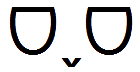
\includegraphics[height=2ex]{Demo_face-removebg-preview .png}}
\usepackage{amsmath}
\usepackage{geometry}
\usepackage{tikz}
\usepackage{float}
\usepackage{graphics}

\tikzset{every picture/.style={line width=0.75pt}} %set default line width to 0.75pt        

\begin{document}
\maketitle
\thispagestyle{empty}
\newpage 

\begin{homeworkProblem}
    Pruebe que los siguientes conjuntos no son algebraicos:
    \begin{itemize}
        \item $\{(z,w)\in A^2(\mathbb{C})\,|\,|z|^2+|w|^2=1\}.$ 
            \begin{solucion}
                Sea $X=\{(z,w)\in A^2(\mathbb{C})\,|\,|z|^2+|w|^2=1\}.$ Suponga que $X$ es un conjunto algebraico, luego existe $ S\subseteq \mathbb{C}[x,y]$, no vació y de polinomios no constantes tal que $X=V(S).$ Sea $f(x,y)=\sum_{i=0}^{m}f_i(y)x^i\in S,$ donde $f_i(y)\in\mathbb{C}[y].$ Consideremos $w_0\in\mathbb{C}$ tal que $|w_0|<1,$ luego $|z|^2=1-|w_0|^2$, luego el polinomio $f(x,w_0)=\sum_{i=0}^{m}f_i(w_0)x^i$ tiene infinitas raíces, ya que hay infinitos puntos en el circulo del plano complejo centrado en $0$ y de radio $1-|w_0|^2.$ Pero esto solo es posible si $f_i(w_0)=0$ para todo $|w_0|<1$ y cada $i=0,1,\ldots,m$, luego como hay infinitos $w_0$ complejos, que cumplen tener norma menor que 1, $f_i=0$ para todo $i=0,1,\ldots,m$, así $f=0,$ pero esto es una contradicción, ya que $f$ por hipótesis es no constante. Así concluimos que $X$ no es algebraico.

                \qed
            \end{solucion}
        \item $\{(\cos(t),\sin(t),t)\in A^3(\mathbb{R})\,|\,t\in\mathbb{R}\}.$
            \begin{solucion}
                Sea $X=\{(\cos(t),\sin(t),t)\in A^3(\mathbb{R})\,|\,t\in\mathbb{R}\}.$ Suponga que $X$ es un conjunto algebraico, luego existe $S\subseteq\mathbb{R}[x,y,z]$, no vació y de polinomios no constantes tal que $X=V(S).$ Sea $f(x,y,z)=\sum_{i=0}^{m}f_i(x,y)z^i\in S,$ donde $f_i(x,y)\in \mathbb{R}[x,y].$ Consideremos $\theta_0\in[0,2\pi)$ luego por la periodicidad del coseno y del seno, note que $f(\cos(\theta_0+2k\pi),\sin(\theta_0+2k\pi),\theta_0+2k\pi)=f(\cos(\theta_0),\sin(\theta_0),\theta_0+2k\pi)=0,$ para todo $k\in\mathbb{Z},$ ya que este ultimo es un punto de $X.$ Así para $\theta_0$ fijo tenemos que $f(\cos(\theta_0),\sin(\theta_0),z)$ tiene infinitas raíces, luego $f_i(\cos(\theta_0),\sin(\theta_0))=0$ para todo $\theta_0\in[0,2\pi)$ y cada $i=0,1,\ldots,m.$ Así cada $f_i$ tiene infinitas raíces, entonces $f_i=0$ para todo $i=0,1,\ldots,m$, luego $f=0,$ llegando así a una contradicción y concluyendo que $X$ no es algebraico.

                \qed 
            \end{solucion}
    \end{itemize}
\end{homeworkProblem}
\newpage
\begin{homeworkProblem}
    Muestre a través de un ejemplo que la unión infinita de algebraicos no siempre es un conjunto algebraico
    \begin{solucion}
        Consideremos $A^1(\R)=\R$ y tomemos $X= \Z \subseteq A^1(\R)$ note que $\Z=\bigcup_{a\in Z}\{a\},$ sabemos que $\{a\}=V(x-a)$, por lo que $\Z$ es la unión contable de conjuntos algebraicos. Si $X$ fuera algebraico existiría $S\subseteq \R[x]$, no vació y de polinomios no constantes, tal que $X=V(S)$, luego dado $f\in S,$ es un polinomio con infinitas raíces ya que todos los enteros son raíces, así $f=0,$ una contradicción. Mostrando así que una unión infinita de conjuntos algebraicos no es un conjunto algebraico siempre.

        \qed
    \end{solucion}
\end{homeworkProblem}

\begin{homeworkProblem}
    Sean $V\subseteq A^n(\K)$ y $W\subseteq A^m(\K)$ conjuntos algebraicos. Demuestre que
    $$V\times W=\{(a_1,\ldots,a_n,b_1,\ldots,b_m)\in A^{n+m}(\K)\,|\,(a_1,\ldots,a_n)\in V,(b_1,\ldots,b_m)\in W\}$$
    es algebraico.
    \begin{solucion}
        Como $V$ y $W$ son algebraicos, existen $S_1\subseteq \K[x_1,\ldots,x_n]$ y $S_2\subseteq \K[y_1,\ldots,y_m],$ no vacíos y de polinomios no constantes tales que $V=V(S_1)$ y $W=V(S_2).$ Definamos los conjuntos $\widehat{S}_1,\widehat{S}_2\subseteq \K[x_1,\ldots,x_n,y_1,\ldots,y_m],$ tales que, dada $\hat{f}\in \widehat{S}_1$, tenemos que $\hat{f}(x_1,\ldots,x_n,y_1,\ldots,y_m)=f(x_1,\ldots,x_n),$ donde $f\in S_1,$ y dada $\hat{g}\in\widehat{S}_2$, tenemos que $\hat{g}(x_1,\ldots,x_n,y_1,\ldots,y_m)=g(y_1,\ldots,y_m),$ donde $g\in S_2.$ Basta con probar que $V\times W=V(\widehat{S}_1\cup\widehat{S}_2).$ Sea $p\in V\times W,$ luego $p=(a_1,\ldots,a_n,b_1,\ldots,b_m),$ donde $(a_1,\ldots,a_n)\in V$ y $(b_1,\ldots,b_m)\in W,$ Note que tomando $h\in \widehat{S}_1\cup\widehat{S}_2 $ tenemos que $h=\hat{f}$ o $h=\hat{g}$, para algún $\hat{f}\in \widehat{S}_1$ o $\hat{g}\in\widehat{S}_2.$\\
        En el primer caso tenemos que $h(p)=\hat{f}(p)=f(a_1,\ldots,a_n)=0,$ ya que $(a_1,\ldots,a_n)\in V(S_1).$ En el otro caso tenemos que $h(p)=\hat{g}(p)=g(b_1,\ldots,b_m)=0,$ ya que $(b_1,\ldots,b_m)\in V(S_2).$ Concluyendo así que para todo $h\in \widehat{S}_1\cup\widehat{S}_2$ tenemos que $h(p)=0$ y por tanto $p\in V(\widehat{S}_1\cup\widehat{S}_2),$ mostrando así que $V\times W\subseteq V(\widehat{S}_1\cup\widehat{S}_2).$ Ahora sea $p\in V(\widehat{S}_1\cup\widehat{S}_2)$ luego para todo $h\in \widehat{S}_1\cup\widehat{S}_2 .$ $h(p)=0.$ Para los $h\in \widehat{S}_1 $ tenemos que $h(p)=\hat{f}(p)=f(p_1,\ldots,p_n).$ Como es arbitrario, tenemos que para todo $f\in S_1,$ $f(p_1,\ldots,p_n)=0,$ es decir, $(p_1,\ldots,p_n)\in V(S_1)=V.$ De manera similar para los $h\in \widehat{S}_2,$ tenemos que $0=h(p)=\hat{g}(p)=g(p_{n+1},\ldots,p_{n+m}),$ concluyendo análogamente que $(p_{n+1},\ldots,p_{n+m})\in V(S_2)=W.$ Luego por como lo definimos concluimos que $p\in V\times W,$ mostrando que $V(\widehat{S}_1\cup\widehat{S}_2) \subseteq V\times W.$ Por la doble continencia, concluimos la igualdad y por tanto que $V\times W$ es algebraico. \qed
    \end{solucion}
\end{homeworkProblem}
\begin{homeworkProblem}
    Calcule las componentes irreducibles de $V(2x^2+3x^2-11,x^2-y^2-3)\subseteq A^2(\C).$
    \begin{solucion}
        Primero notemos que $V:=V(2x^2+3x^2-11,x^2-y^2-3)=V(2x^2+3x^2-11)\cap V(x^2-y^2-3).$ Luego dado $(x,y)\in V,$ tiene que ser solución del siguiente sistema de ecuaciones
        $$
            \begin{cases}
                2x^2+3x^2-11=0,\\
                x^2-y^2-3=0.
            \end{cases}
        $$
        Multiplicando la segunda ecuación por 3 y sumando ambas ecuaciones obtenemos
        \begin{align*}
            0&=2x^2+3x^2-11+3x^2-3y^2-9\\
            &=5x^2-20,
        \end{align*}
         esta ecuación se satisface si $x=2$ o $x=-2.$ Para hallar $y$, reemplazamos los valores de $x$ en $x^2-y^2-3=0,$ así
         $$(2)^2-y^2-3=(-2)^2-y^2-3=1-y^2=0.$$
         Por lo tanto $y=1$ o $y=-1,$ así concluimos que $V=\{(2,1)\}\cup\{(2,-1)\}\cup\{(-2,1)\}\cup\{(-2,-1)\}.$ Es decir las componentes irreducibles de $V(2x^2+3x^2-11,x^2-y^2-3)$ son $V_1=\{(2,1)\},V_2=\{(2,-1)\},V_3=\{(-2,1)\}$ y $V_4=\{(-2,-1)\}.$
         
         \qed
    \end{solucion}
\end{homeworkProblem}

%%%%%%%%%%%%%%%%%%%%%%%%%%%%%%%%%%%%%%%%%%%%%%%%%%%%%%%
\end{document}